% Description: TD Base de données - Initiation à PostgreSQL

% Preamble
\documentclass[11pt]{article}
\usepackage[utf8]{inputenc}
\usepackage[T1]{fontenc}
\usepackage[francais]{babel} % pour la syntaxe du texte en français
\usepackage[table]{xcolor} % pour les tableaux
\usepackage{graphicx} % pour les images
\usepackage{float} % pour le positionnnement des images et tableaux
\usepackage{hyperref} % pour les liens hypertexte
\usepackage{fancyhdr} % pour la mise en page (entête, pied de page)

\usepackage{listings} % pour l'insertion de texte brut, de code
\usepackage{color}
\lstset{
	language=SQL,
	showspaces=false,
	breaklines=true,
	basicstyle=\small\ttfamily,
	numbers=none,
	commentstyle=\color{purple}\small\sffamily,
	frame=lrbt,
	frameround=tttt
}

\usepackage{vmargin} % gestion des marges, hauteurs de pieds de page...
\setmargins{3.5cm}			% Gauche
					 {1.5cm}			% Haut
					 {14.7cm}			% Largeur du texte
					 {23.42cm}		% Hauteur du texte
					 {14pt}				% Hauteur entête
					 {1cm}				% Distance entête
					 {0pt}				% Hauteur pied de page
					 {2cm}				% Distance pied de page

\usepackage{titlesec} % gestion des espaces entre paragraphes
\titlespacing{\subsection}{0pt}{1cm}{0cm}
\titlespacing{\subsubsection}{0pt}{0.5cm}{0cm}
		   
\setlength{\parskip}{1em}
\renewcommand{\floatpagefraction}{1} % permet d'avoir plusieurs grandes images sur une page
\parindent=0cm % suppression de la tabulation pour la 1ère ligne des paragraphes



% infos sur le document
\title{Introduction aux bases de données\\Initiation à PostgreSQL}
\author{Clément Delgrange}
\date{\today}
	


% Document
\begin{document}

	% Définition des entêtes et pieds de page
	\pagestyle{fancy}
	\fancyhf{}
	\renewcommand{\headrulewidth}{0pt}
	\fancyfoot[L]{TD Bases de données}
	\fancyfoot[C]{-\thepage-}
	\fancyfoot[R]{C. Delgrange}
	\renewcommand{\footrulewidth}{0.5pt}

	

	% Page de titre
	\begin{titlepage}
		\begin{sffamily}
			\begin{flushleft}
				
\includegraphics[scale=0.15]{../images/logo_ensg.png}\\[1.5cm]
			\end{flushleft}
			\begin{flushright}
				% pour mettre une image en haut à droite
			\end{flushright}
			
			\begin{center}
				\hrule
					\vspace{0.5cm}
					{\LARGE \bfseries TD Bases de données}
					\vspace{0.7cm}
				\hrule
				
				\vspace{3cm}
				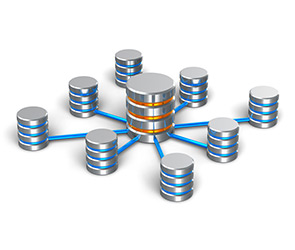
\includegraphics[scale=0.75]{../images/bdd.jpg}
				\vspace{3.5cm}
			
				\large \textit{Clément Delgrange\\
				Octobre 2015}
			\end{center}
		\end{sffamily}
	\end{titlepage}
	
	
	
	\section*{Introduction}
	\label{sec:Introduction}
		L'objectif de ce TD est de concevoir puis utiliser une base de données destinée à la gestion de l'alimentation des animaux d'un zoo. Le nom donné à cette base sera ZOO. On utilisera le SGBD (Système de Gestion de Bases de Données) PostgreSQL et son interface d'administration PgAdmin.
	
		L'analyse de la problématique puis la réalisation du modèle conceptuel de données ont été réalisés lors d'un précédent exercice. 
	
	
	\section{Rappel / définitions}
	Base de données = ensemble de données qui sont stockées sur un support informatique, et organisées et structurées de manière à pouvoir facilement consulter et modifier leur contenu.
	
	SGBD = logiciel permettant de manipuler une base de données
	
	SGBDR = SGBD permettant de manipuler une base de données relationnelle
	
	Modèle conceptuel de données = schéma décrivant de façon formelle les objets qui seront utilisées dans le système d'information et les liens entre ces objets, en faisant abstraction des solutions et contraintes techniques d'implémentation de la base de données.
	
	Modèle relationnel de données = modèle basé sur une organisation des données sous forme de tables, encore appelées relations. Chaque relation est constituée d'une en-tête et de ligne. Le modèle relationnel permet de mettre en oeuvre des opérations élémentaires sur les relations (intersection, union, différence).
	
	
	
	\section{Réalisation du modèle relationnel}
		Avant de commencer à enregistrer la base dans le SGBD, terminez la phase de préparation en traduisant le modèle conceptuel de données en modèle relationnel.
		
		Vous repartirez pour cette modélisation du modèle conceptuel ci-dessous :
		\begin{figure}[H]
			\center 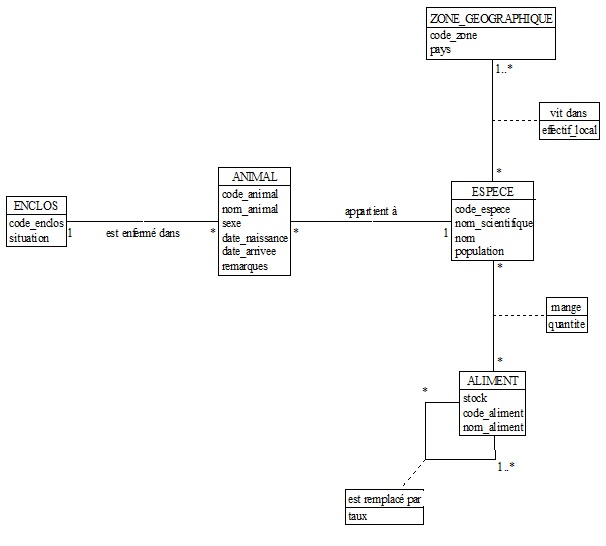
\includegraphics[width=0.8\textwidth]{../images/MCD.jpg}\\[1em]
		\end{figure}
		
		
	\section{Création de la base de données}
		On utilisera pour l'instant PgAdmin pour manipuler notre base de données. PgAdmin est un outil d'administration graphique pour PostgreSQL.
		
		Son interface se présente de la manière suivante :
		\begin{figure}[H]
			\center 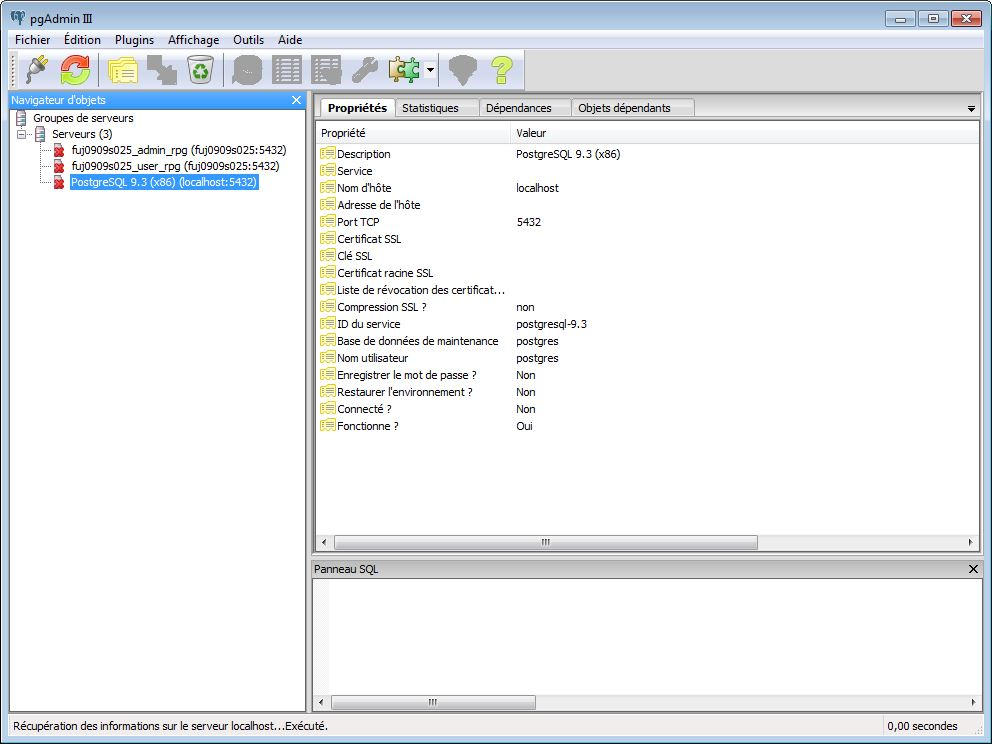
\includegraphics[width=0.8\textwidth]{../images/pgadmin.jpg}\\[1em]
		\end{figure}
		
		Sur la gauche, dans la partie \textit{Navigateur d'objets}, on retrouve la liste des serveurs avec lesquels une connexion a été enregistrée. Ils sont barrés d'une petite croix rouge si aucune connexion n'a encore été établie dans la session en cours.
		
		$\Rightarrow$ Connectez vous au serveur \textit{localhost} en double cliquant dessus puis dépliez l'item \textit{Bases de données}. 
		
		Cela permet d'afficher la liste des bases de données stockées sur le serveur \textit{localhost} (ie. le poste sur lequel vous travaillez).
		\begin{figure}[H]
			\center \includegraphics[width=0.4\textwidth]{../images/pgadmin_navigateur.jpg}\\[1em]
		\end{figure}
		
		$\Rightarrow$ Ajoutez une nouvelle base de données à l'aide d'un clic droit sur \textit{Bases de données > Ajouter une base de données...}. Nommez la \textbf{ZOO}.
		\begin{figure}[H]
			\center 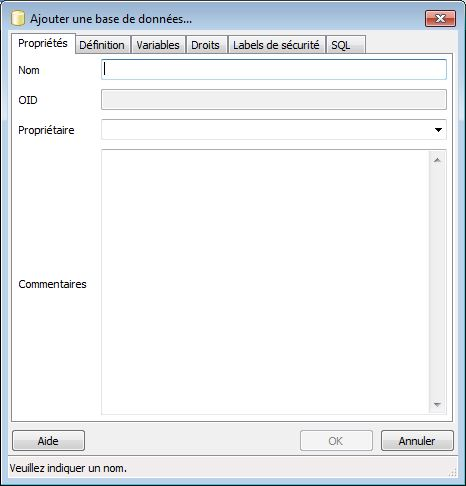
\includegraphics[width=0.6\textwidth]{../images/pgadmin_ajouter_base.jpg}\\[1em]
		\end{figure}
		
		En dépliant la base de données créée, on obtient :
		\begin{figure}[H]
			\center 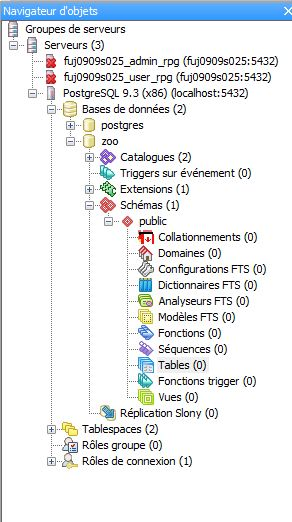
\includegraphics[width=0.35\textwidth]{../images/pgadmin_base_cree.jpg}\\[1em]
		\end{figure}
	
	
	\section{Création des tables}
		\subsection{Table ALIMENT}
			$\Rightarrow$ Dépliez le schéma \textit{public} et, par clic droit sur \textit{Tables}, ajoutez une nouvelle table.
			\begin{figure}[H]
				\center 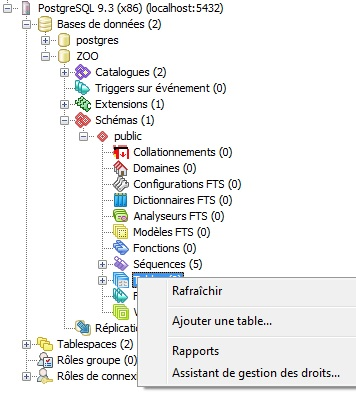
\includegraphics[width=0.45\textwidth]{../images/pgadmin_ajouter_table-1.jpg}\\[1em]
			\end{figure}
			
			$\Rightarrow$ Nommez votre table \textbf{ALIMENT}
			\begin{figure}[H]
				\center 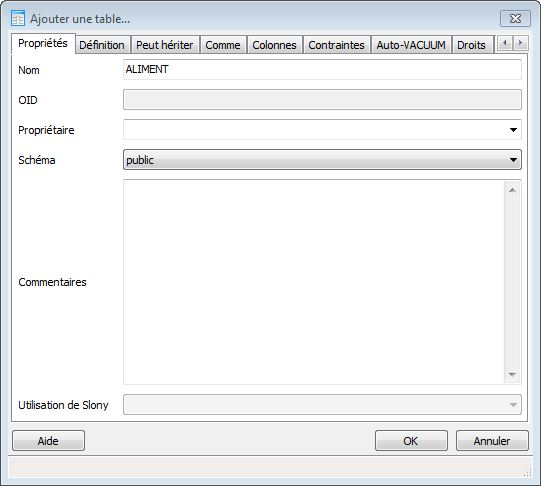
\includegraphics[width=0.6\textwidth]{../images/pgadmin_ajouter_table-2.jpg}\\[1em]
			\end{figure}
			
			$\Rightarrow$ Dans l'onglet \textit{Colonnes}, ajoutez les colonnes \textbf{code\_aliment} de type serial, \textbf{nom\_aliment} de type Text et \textbf{stock} de type entier.
			\begin{figure}[H]
				\center 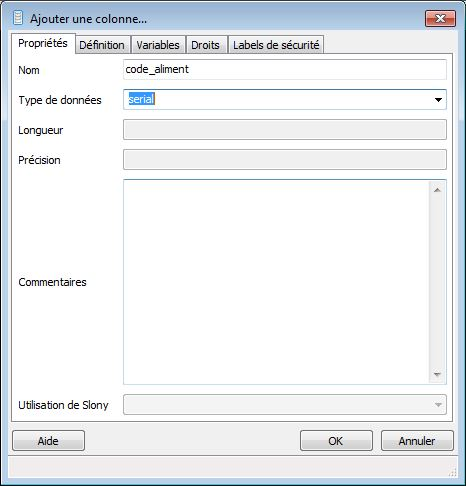
\includegraphics[width=0.6\textwidth]{../images/pgadmin_ajouter_colonne.jpg}\\[1em]
			\end{figure}
			
			Le type serial est un type numérique spécifique à PostgreSQL. Il permet de définir un entier qui s'auto-incrémente lorsque des enregistrement sont ajoutés à la table. Il est particulièrement adapté pour des identifiants uniques de table.
			
			\fbox{
				\begin{minipage}{0.9\textwidth}
					Les types de données couramment utilisés dans Postgres sont : 
					\begin{itemize}
						\item numériques : smallint, integer, bigint (entiers plus ou moins longs), decimal, numeric, real, double precision (nombres à virgules plus ou moins précis), serial (entier auto-incrémenté);
						\item monétaire;
						\item caractères : character, char, text (qui se différencient par le nombre de caractères autorisés);
						\item binaire;
						\item date/heure : date, heure, date-heure, intervalle;
						\item booleen (valeurs possibles : TRUE, t, true, y, yes, on, 1 / FALSE, f, false, n, no, off, 0);
						\item géométriques : point, line, lseg, box, path, polygon, circle;
						\item adresse réseau : IPv4, IPv6 et MAC;
						\item types composites (listes de types simples, peu recommandées).
					\end{itemize}
				\end{minipage}
			}
			\vspace{1em}
			
			$\Rightarrow$ Enfin, dans l'onglet \textit{Contrainte}, ajoutez une clé primaire \textit{code\_aliment\_cle\_primaire}. Faite portez cette clé primaire sur le champs \textbf{code\_aliment} (sélectionnez la colonne adéquat dans l'onglet \textit{Colonnes}).
			
			\textbf{Une clé primaire permet de distinguer de façon unique les éléments d'une table. La clé primaire peut être composée d'une ou de plusieurs colonnes.} 
			
			$\Rightarrow$ Le paramétrage de la table est maintenant terminé : validez sa création.
			\begin{figure}[H]
				\center 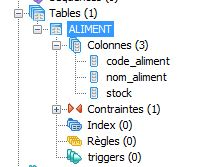
\includegraphics[width=0.4\textwidth]{../images/pgadmin_table_aliment.jpg}\\[1em]
			\end{figure}
			
			$\Rightarrow$ Retournez dans l'explorateur pour sélectionner la table.
			
			Cela fait apparaître des instructions dans le \textit{Panneau SQL} de PgAdmin :
			\begin{figure}[H]
				\center 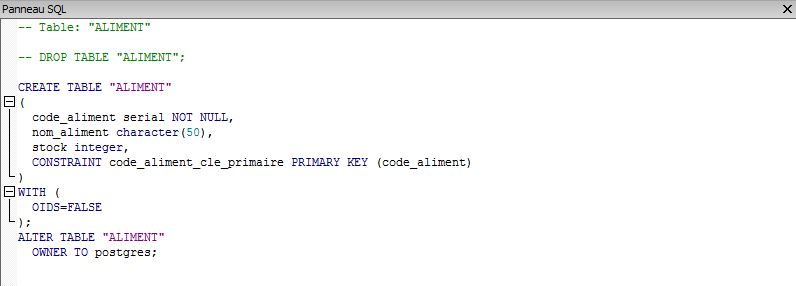
\includegraphics[width=0.8\textwidth]{../images/pgadmin_panneau_sql.jpg}\\[1em]
			\end{figure}
			
			Il s'agit des instructions SQL de création de la table \textbf{ALIMENT}.
			
			\textbf{Le SQL (Structured Query Language) est un langage informatique normalisé servant à interagir avec des bases de données relationnelles.} C'est le langage pour base de données le plus répandu, même si l'on peut observer quelques petites différences d'implémentation selon les SGBDR.
			
			$\Rightarrow$ A partir de cet exemple d'instruction SQL, déduire la syntaxe générique de création d'une table en SQL.
			
			......................................................................\\
			......................................................................\\
			......................................................................\\
			......................................................................\\
			......................................................................\\
			
			\subsection{Table ENCLOS}
				$\Rightarrow$ Dans la barre d'outils de PgAdmin, cliquez sur le bouton d'ouverture du constructeur de requêtes SQL.
				\begin{figure}[H]
					\center 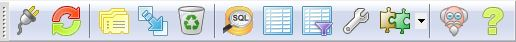
\includegraphics[width=0.7\textwidth]{../images/pgadmin_barre_outils.jpg}\\[1em]
				\end{figure}
				 
				Le constructeur de requêtes permet d'écrire des instructions en SQL pour les envoyer à la base de données.
				
				$\Rightarrow$ A l'aide d'une requête SQL créez la table \textbf{Famille}. Elle comportera deux colonnes : \textbf{code\_enclos} de type serial et \textbf{situation} de type text, et une clé primaire.

			\subsection{Table ESPECE}
				$\Rightarrow$ De la même manière, créez la table Enclos. 
				
				Elle comportera 4 colonnes : \textbf{code\_espece} de type serial, \textbf{nom} de type varchar(50), \textbf{nom\_scientifique} de type varchar(50) et \textbf{population} de type integer. Elle contriendra également une clé primaire sur la colonne code\_espece.
			
			
			\subsection{Table ANIMAL}
				$\Rightarrow$ De la même manière, créez la table ANIMAL. Elle comportera 6 colonnes :
				\begin{itemize}
					\item \textbf{code\_animal} de type serial
					\item \textbf{nom\_animal} de type varchar(50) 
					\item \textbf{sexe} de type char
					\item \textbf{date\_naissance} de type date
					\item \textbf{date\_arrivee} de type date
					\item \textbf{remarques} de type texte
				\end{itemize}
				
				Elle comportera également une clé primaire sur la colonne code\_animal.
				
				Par ailleurs, pour représenter la relation entre les tables ANIMAL et ENCLOS d'une part et ANIMAL et ESPECE d'autre part, nous ajouterons deux colonnes dans la table :
				\begin{itemize}
					\item \textbf{code\_espece} de type integer
					\item \textbf{code\_enclos} de type integer
				\end{itemize}
				
				Ces deux colonnes pointerons vers les colonnes de même nom des tables ESPECE et ENCLOS. Pour s'assurer que les identifiants saisis dans ces colonnes soient bien présent dans les tables d'origine, nous ajouterons des clés étrangères.
				
				\textbf{Les clés étrangères permettent de gérer les relations entre plusieurs tables. Elles garantissent la cohérence des données.}

			
			\subsection{Autres tables du modèle}
				Complétez la base avec les tables pas encore implémentées du modèle relationnel : ZONE\_GEOGRAPHIQUE, ALI\_SUBSTITUTION, ESP\_ANI et ESP\_ZONEGEO.
						

			\subsection{Modification de la structure de la base}
				La base que nous avons implémenté jusqu'à présent ne tient pas compte de toute les contraintes prévues dans le modèle conceptuel.
				
				On peut modifier une table en utilisant une instruction \lstinline{ALTER TABLE ...}. Par exemple pour ajouter une condition \lstinline{NOT NULL} sur la colonne stock de la table ALIMENT, on exécutera l'instruction SQL :
				\begin{lstlisting}
ALTER TABLE "ALIMENT" ALTER COLUMN "stock" SET NON NULL
				\end{lstlisting}
				
				$\Rightarrow$ Recopiez et exécutez cette instruction.
				
				$\Rightarrow$ De manière similaire, écrivez et exécutez les instructions permettant de ajouter les conditions suivantes dans la base :
				\begin{itemize}
					\item Table ANIMAL, code\_espece non nul
					\item Table ESPECE, nom\_scientifique non nul
					\item Table ESP\_ALI, quantite non nulle
					\item Table ZONE\_GEOGRAPHIQUE, pays non nul
				\end{itemize}
				
				On souhaite également ajouter une contrainte sur la table ANIMAL pour s'assurer que la date de naissance est postérieure à la date d'arrivée. La syntaxe est :
				\begin{lstlisting}
ALTER TABLE "ANIMAL" ADD CONSTRAINT nom_contrainte contrainte
				\end{lstlisting}
				
				$\Rightarrow$ Ajoutez une contrainte date\_naissance > date\_arrivee
				
				Le libellé initialement choisi pour la colonne quantite de la table des aliments de substitution apparait finalement mal choisi et on souhaite le modifier. Pour renommez une colonne, la structure de l'instruction SQL sera de type :
				\begin{lstlisting}
ALTER TABLE nom_table RENAME COLUMN colonne TO nouvelle_colonne
				\end{lstlisting}
				
				$\Rightarrow$ Dans la table ALI\_SUBSTITUTION, renommez la colonne quantite en taux et ajoutez une contrainte non nul sur cette colonne.
				
				
		\section{Insertion des données}
			\subsection{Dans PgAdmin}
				Maintenant que la structure de notre base est en place, il est temps de commencer à y insérer des enregistrements. Dans PgAdmin, cette opération peut s'effectuer en ouvrant la fenêtre d'édition des données : sélectionner la table dans le navigateur d'objets et cliquer sur le bouton d'ouverture de la fenêtre.
				
				\begin{figure}[H]
					\center 
\includegraphics[width=0.07\textwidth]{../images/pgadmin_bouton_edition_donnees.jpg}\\[1em]
				\end{figure}
				
				L'interface est alors très similaire à un tableau excel. 
				
				$\Rightarrow$ Ajoutez 5 lignes à la table ENCLOS en respectant les éléments de la capture d'écran ci-dessous :
				
				\begin{figure}[H]
					\center 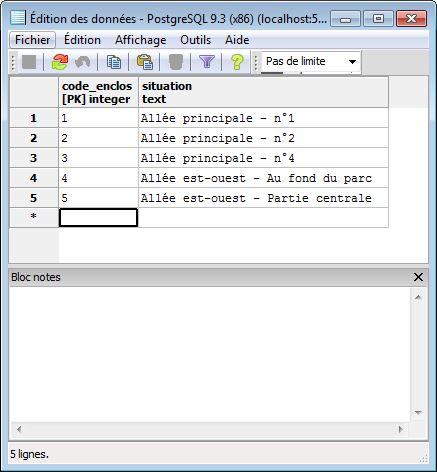
\includegraphics[width=0.7\textwidth]{../images/pgadmin_fenetre_edition.jpg}\\[1em]
				\end{figure}
				
				
			\subsection{A l'aide d'une requête SQL}
				L'insertion d'enregistrement est bien évidemment également accessible en SQL. La syntaxe est :
				\begin{lstlisting}
INSERT INTO table ([colonne1, colonne2, ...]) VALUES (expression1, expression2, ...);
				\end{lstlisting}
				
				$\Rightarrow$ Recopiez la ligne suivante pour insérer une ligne dans la table ALIMENT :
				\begin{lstlisting}
INSERT INTO "ALIMENT" ("code_aliment", "nom", "stock") VALUES (1, "Ble", 100);
				\end{lstlisting}
				
				$\Rightarrow$ Insérez ensuite les lignes suivantes dans la table ALIMENT :
				
				\begin{center}
					\begin{tabular}{c|l|c}
						\textbf{code\_aliment} & \textbf{nom} & \textbf{stock} \\
						\hline
						2 & Foin & 75 \\
						3 & Herbe & 450 \\
						4 & Poisson & 47 \\
						5 & Bananes & 32 \\
						6 & Bambou & 79 \\
						7 & Insectes & 13 \\
						8 & Viande & 27 \\
						9 & Carcasse animale & 50 \\
						10 & Baies & 4 \\
						11 & Carottes & 30 \\
					\end{tabular}
				\end{center}
				
				
			\subsection{A l'aide d'un fichier .sql}
				L'insertion manuelle de l'ensemble des données de la base serait assez fastidieuse. Heureusement, PostgreSQL nous met à disposition des outils pour exécuter sur un serveur un ensemble d'instructions SQL contenues dans un fichier. Nous utiliserons cette possibilité pour charger une base ZOO complète.
				
				$\Rightarrow$ Dans PgAdmin renommez votre base ZOO en ZOO2.
				
				$\Rightarrow$ Récuperez le fichier ZOO.sql. Il contient l'ensemble des instruction SQL pour créer la base, les tables, contraintes... et de peupler la base.
				
				PostgreSQL est livré avec un ensemble d'utilitaires (on parle aussi d'applications client de PostgreSQL) qui permettent de manipuler une base de données sur n'import quel serveur sans avoir à ouvrir d'instance de PgAdmin ou à écrire d'instruction SQL. L'autre avantage des ces utilitaires est qu'ils sont identiques sur l'ensemble des plateformes où un client PostgreSQL est installé.
				
				Nous utiliserons ces utilitaires pour créer une nouvelle base de données vierge puis la remplir à l'aide des instructions du fichier ZOO.sql.
				
				$\Rightarrow$ Ouvrez un terminal windows et tapez la commande \lstinline{cd "C:\Program Files (x86)\PostgreSQL\9.3\bin"} pour vous placez dans le répertoire contenant les utilitaires de PostgreSQL 9.3.
				
				$\Rightarrow$ Saisissez ensuite : \lstinline{createdb.exe -h localhost -p 5432 -U postgres ZOO} pour créer une nouvelle base vierge ZOO.
				
				Lors de l'appel à l'outil, on a précisé quelques options :
				\begin{itemize}
					\item h (host) = localhost : on se connecte au serveur local
					\item p (port) = 5432 : port par défaut utilisé par postgres
					\item U (user) = postgres : nom de l'utilisateur avec lequel on se connecte à la base.
				\end{itemize}
				
				Le paramétrage de options se fait de la même manière pour l'ensemble des utilitaires PostgreSQL.
				
				$\Rightarrow$ Saisissez ensuite la ligne \lstinline{psql.exe -h localhost -p 5432 -U postgres -f D:\G1_Bases_de_donnees\ZOO.sql} en remplaçant le chemin par le chemin du fichier ZOO.sql sur votre poste.

				Elle permet d'appeler l'utilitaire psql qui est utilisé pour envoyer des requêtes SQL à un serveur PostgreSQL. L'outil psql accepte en entrée une instruction SQL simple ou un fichier .sql contenant un ensemble d'instruction. 
				
				Retournez dans PgAdmin pour vérifier que la base a correctement été créée et remplie.
				
				
		\section{Sélection de données}
			\subsection{Requêtes SELECT simples}
				La conception de la base étant maintenant achevée, il nous est possible de l'exploiter.
				
				Le mot clé \lstinline{SELECT} permet la sélection et l'affichage de données. Testez par exemple :
				\begin{lstlisting}
SELECT 'Hello world !';
SELECT 2+3;
				\end{lstlisting}
				
				On souhaite d'abord connaître l'ensemble des animaux du zoo.\\
				$\Rightarrow$ Recopiez la requête suivante et observez le résultat :
				\begin{lstlisting}
SELECT * FROM "ANIMAL";
				\end{lstlisting}
				
				$\Rightarrow$ Sélectionnez de la même manière l'ensemble des espèces enregistrées dans la base.
				
				Il peut être intéressant de ne pas afficher toutes les colonnes dans le résultat de la requête. Dans ce cas, on nomme explicitement les colonnes que l'on souhaite afficher.\\
				$\Rightarrow$ Recopiez la requête suivante et observez le résultat :
				\begin{lstlisting}
SELECT "nom", "sexe", "date_naissance" FROM "ANIMAL";
				\end{lstlisting}
				
				$\Rightarrow$ Sur le même principe, affichez les colonnes nom et population de la table ESPECE
			
				Le langage SQL offre aussi la possibilité de renommer une colonne lors de l'affichage du résultat :\\
				$\Rightarrow$ Recopiez la requête suivante et observez le résultat :
				\begin{lstlisting}
SELECT "nom" AS "Nom", "sexe" AS "Sexe", "date_naissance" AS "Date de naissance" FROM "ANIMAL";
				\end{lstlisting}
				 
				$\Rightarrow$ De manière similaire, affichez les colonnes \textit{nom} et \textit{nom\_scientifique} de la table ESPECE en les renommant respectivement en \textit{Nom} et \textit{Nom scientifique}.
				
				
			\subsection{La clause WHERE}
				Il est possible de restreindre le résultat d'une requête avec le mot clé \lstinline{WHERE}.\\
				$\Rightarrow$ Par exemple, la requête suivante sélectionne les animaux né avant 2000.
				\begin{lstlisting}
SELECT * FROM "ANIMAL" WHERE "date_naissance" < '2000-01-01';
				\end{lstlisting}
				
				$\Rightarrow$ En utilisant une clause \lstinline{WHERE}, sélectionnez les espèces dont la population est inférieure à 10000.
				
				L'opérateur de comparaison pour les chaînes de caractères est \textit{like} :\\
				\begin{lstlisting}
SELECT * FROM "ANIMAL" WHERE "sexe" like 'M';
				\end{lstlisting}
				
				\begin{center}
					\begin{tabular}{c|c}
						\textbf{Opérateur} & \textbf{Signification} \\
						\hline
						$=$ & égal \\
						$<$ & inférieur \\
						$<=$ & inférieur ou égal \\
						$>$ & supérieur \\
						$>=$ & supérieur ou égal \\
						$<>$ ou $!=$ & différent \\
						$<=>$ & égal (valable aussi pour \lstinline{NULL}) \\
					\end{tabular}
				\end{center}
				
				$\Rightarrow$ Sélectionnez la ligne de l'espèce tigre.
				
				$\Rightarrow$ Créez une requête pour afficher les colonnes \textit{nom} et \textit{population} des espèces ayant une population supérieure à 100000.
				
				
				Pour des résultats plus évolués, on peut combiner différents critères. Par exemple pour sélectionner les animaux "éléphant" (code\_espece = 2) et "girafe" (code\_espece = 4) :
				\begin{lstlisting}
SELECT "nom", "sexe", "date_naissance", "date_arrivee" FROM "ANIMAL" WHERE code_espece = 2 OR code_espece = 4;
				\end{lstlisting}
				
				\begin{center}
					\begin{tabular}{c|c}
						\textbf{Opérateur} & \textbf{Signification} \\
						\hline
						\lstinline{AND} & ET \\
						\lstinline{OR} & OU \\
						\lstinline{NOT} & NON \\
					\end{tabular}
				\end{center}
				
				$\Rightarrow$ Affichez le nom et la date d'arrivée au zoo (titre de colonne renommé en "Date d'arrivée") des animaux de sexe féminin arrivés dans le zoo avant 2010.
				
				$\Rightarrow$ Sélectionnez les animaux qui sont soit des mâles, soit des girafes (code\_espece = 4), mais pas les deux en même temps.
				
				$\Rightarrow$ Imaginons maintenant une autre requête un peu plus complexe qui nous permette de sélectionner les éléphants nés avant 2000 et les animaux de toutes les autres espèces qui soient nés arrivées au zoo avant 2007 pour les femelles et avant 2005 pour les mâles.
				
			\subsection{Clauses WHERE évoluées}
				Les clauses \lstinline{WHERE} que nous avons utilisé jusqu'ici permettent de tester des conditions simples : égalité, inférieur, supérieur. Mais qu'en est-il si nous souhaitons sélectionner les animaux dont le nom commence par la lettre T. 

				Par ailleurs, la sélection de ceux arrivés au parc entre 2000 et 2005, ou bien de ceux dont le code\_espece est 1, 3 ou 6, est possible avec les expressions déjà introduites, mais la syntaxe résultante sera assez lourde à mettre en place.
				
				Le SQL nous met à disposition des expression pour ce genre de requêtes. Pour les tests sur les chaînes de caractères, on peut utiliser le mot clé \lstinline{LIKE} ("comme") qui permet de tester si une chaîne de caractère ressemble à une autre :
				\begin{lstlisting}
SELECT * FROM table WHERE colonne LIKE valeur;				
				\end{lstlisting}
				
				La valeur testée peut contenir les symboles \_ pour remplacer un caractère inconnu, ou \% pour remplacer plusieurs caractères inconnus.
				
				$\Rightarrow$ Sélectionnez les animaux dont le nom commence par T :
				\begin{lstlisting}
SELECT * FROM "ANIMAL" WHERE "nom" LIKE 'T%';				
				\end{lstlisting}
			
				$\Rightarrow$ De la même manière, sélectionnez les animaux dont le nom comporte 'ou'.
				
				Pour tester si une colonne est comprise entre deux valeurs on peut utiliser \lstinline{BETWEEN(valeur_min, valeur_max)}. Pour tester si elle est dans une plage de valeurs, on utiliser \lstinline{IN(valeur1, valeur2, ...)}
				
				$\Rightarrow$ Sélectionnez les animaux dont le nom commence par T, C ou B.
				
				$\Rightarrow$ Sélectionnez les animaux arrivés au parc entre 2005 et 2010.
			
			
			\subsection{Tri des données}
				Jusqu'à présent, lorsque l'on a exécuté une requête \lstinline{SELECT}, les lignes sélectionnées sont retournées dans un ordre défini par PostgreSQL et qui n'a pas forcément de sens pour nous. Or il arrivera fréquemment que l'on veuille trier nous même le résultat de la requête. On utilisera pour cela \lstinline{ORDER BY colonne} à la fin de la requête.
				
				$\Rightarrow$ Sélectionnez les éléphants en ordonnant le résultat par ordre alphabétique.
				
				Pour inverser l'ordre de la sélection, on utilise le mot clé \lstinline{DESC} :
				\begin{lstlisting}
SELECT "nom", "sexe", "date_naissance" FROM "ANIMAL" ORDER BY "date_naissance" DESC;
				\end{lstlisting}
				
				On peut également trier sur plusieurs colonnes : \lstinline{ORDER BY colonne1, colonne2}.
				
				$\Rightarrow$ Sélectionnez les animaux en triant le résultat par ordre d'arrivée dans le zoo et en cas d'arrivées le même jour, en mettant l'animal le plus vieux en premier.
				
			
			\subsection{Limiter les résultats}
				Sur les grosses bases de données, le nombre de résultats retournés par une requête de sélection peut être énorme et faire baisser les performances de la machine. Aussi, pour limiter l'affichage à un nombre donné de ligne, on peut utiliser la clause \lstinline{LIMIT} :
				\begin{lstlisting}
LIMIT nombre_de_ligne [OFFSET decalage];
				\end{lstlisting}
				
				$\Rightarrow$ Testez les deux requêtes suivantes pour comprendre le fonctionnement de la clause \lstinline{LIMIT} :
				\begin{lstlisting}
SELECT * FROM "ANIMAL" ORDER BY "nom";

SELECT * FROM "ANIMAL" ORDER BY "nom" LIMIT 4 OFFSET 2;
				\end{lstlisting}
			
				$\Rightarrow$ Affichez le nom des 3 animaux les plus jeunes du zoo.
				
			
			\subsection{Eliminer les doublons}
				Si l'on exécute une requête \lstinline{SELECT "code_espece" FROM "ANIMAL";} pour récupérer la liste des codes espèce des animaux du zoo, le résultat nous présentera plusieurs fois le même code si plusieurs animaux de la même espèce sont présents. Cela ne sera pas très exploitable.
				
				Pour supprimer les doublons de l'affichage, on peut utiliser le mot clé \lstinline{DISTINCT}, placé juste après le \lstinline{SELECT}.
				
				$\Rightarrow$ Affichez la liste des codes espèce des animaux présent dans le zoo en éliminant les doublons.
				
				On peut également utiliser l'option \lstinline{GROUP BY (colonne1, colonne2...)} pour fusionner les résultats ayant les mêmes valeurs dans une colonne ou un groupe de colonnes données.
				
				$\Rightarrow$ Testez les requête :
				\begin{lstlisting}
SELECT "code_espece" FROM "ANIMAL";

SELECT "code_espece" FROM "ANIMAL" GROUP BY "code_espece";
				\end{lstlisting}
				
				Cette seconde option permet, en plus, d'effectuer des comptages sur les résultats :
				\begin{itemize}
					\item \lstinline{count(*)} : compte le nombre de lignes regroupées
					\item \lstinline{sum(colonne)} : fait la somme des valeurs de la colonne indiquée pour les lignes regroupées
					\item ...
				\end{itemize}
				Ces comptages s'affichent comme des colonnes classiques dans la requête.
				
				$\Rightarrow$ Pour comprendre le fonctionnement, testez la requête :
				\begin{lstlisting}
SELECT "code_espece", count(*) AS "Nombre" FROM "ANIMAL" GROUP BY "code_espece";
				\end{lstlisting}
				
				$\Rightarrow$ Pour chaque espèce, affichez le nombre d'aliment qu'elle mange et la quantité totale que cela représente.
			
			
			
		\section{Jointures}
			Jusqu'à présent nous avons uniquement manipulé les tables unes à unes. Mais l'utilisation des bases de données ne se limite à cela. Elles permettent en effet de mettre les tables en relation et de croiser les informations pour effectuer certaines analyses. On parlera de jointures.
		
			Il existe plusieurs types de jointures. Le premier que nous allons voir est la jointure interne.
		
			$\Rightarrow$ Observez le résultat de la requête :
			\begin{lstlisting}
SELECT "ANIMAL"."nom", "ANIMAL"."code_espece", "ESPECE"."nom" 
FROM "ANIMAL" INNER JOIN "ESPECE" ON "ANIMAL"."code_espece" = "ESPECE"."code_espece";
			\end{lstlisting}
			
			$\Rightarrow$ Affichez le nom de chaque animal, le numéro de son enclos et la situation de l'enclos.
			
			Si l'on revient sur la première jointure, le résultat fait apparaître deux colonnes \textit{nom}, ce qui peut n'est pas très pratique pour une exploitation future. On prendra donc soin d'utiliser pertinemment des alias.
			
			$\Rightarrow$ Ré-écrivez la requête en renommant les champs en sortie.
			
			On peut également utiliser des alias pour renommer les tables et ainsi avoir moins de code à écrire :
			\begin{lstlisting}
SELECT "A"."nom", "E"."nom" 
FROM "ANIMAL" AS "A" INNER JOIN "ESPECE" AS "E" ON "A"."code_espece" = "E"."code_espece";
			\end{lstlisting}
			
			$\Rightarrow$ Sélectionnez le nom des animaux dont la population de l'espèce est inférieure à 50000.
			
			La jointure interne ne permet de sélectionner que les lignes qui correspondent dans les deux tables. Pour sélectionner tous les éléments de la table de référence (aussi appelée table de gauche) et ceux correspondant de la table jointe (ou table de droite), on effectue une jointure par la droite.
			
			La jointure inverse (jointure par la gauche) est également possible.
			
			$\Rightarrow$ Testez et comparez :
			\begin{lstlisting}
SELECT "A"."nom"
FROM "ALIMENT" AS "A" INNER JOIN "ESP_ALI" AS "EA" ON "A"."code_aliment" = "EA"."code_aliment";

SELECT "A"."nom"
FROM "ALIMENT" AS "A" LEFT JOIN "ESP_ALI" AS "EA" ON "A"."code_aliment" = "EA"."code_aliment";
			
SELECT "A"."nom", "EA"."quantite", "EA"."code_espece"
FROM "ALIMENT" AS "A" LEFT JOIN "ESP_ALI" AS "EA" ON "A"."code_aliment" = "EA"."code_aliment";
			\end{lstlisting}
			
			$\Rightarrow$ Affichez les noms des animaux vivant dans chaque enclos, avec la situation de l'enclos. Les enclos vide doivent apparaître dans la liste. Triez le résultat par numéro d'enclos.
			
			Il est possible d'effectuer plusieurs jointures dans la même requête :
			
			$\Rightarrow$ Affichez la table ALI\_SUBSTITUTION en remplaçant code\_aliment et code\_substitution par le nom de l'aliment.
			
			\underline{Un petit problème...}
			
			Pour optimiser les tournées du personnel nourrissant les animaux, on désire connaître à l'avance les quantités et types de nourriture à apporter dans un enclos donné.
			
			$\Rightarrow$ Dans un premier temps, sélectionnez tous les animaux de l'enclos 2. Affichez leur nom, les aliments qu'ils consomment et la quantité consommée.
			
			$\Rightarrow$ Affinez la requête pour afficher la quantité consommée par type d'aliment.
			On souhaite maintenant savoir si les stocks d'aliments sont suffisant pour nourrir tous les animaux du zoo.
			
			\underline{Un second problème...}
			
			On souhaite maintenant savoir quels sont les aliments pour lesquels le stock est inférieur à la quantité consommée.
			
			$\Rightarrow$ Pour commencer, afficher pour chaque animal : son nom, les noms des aliments qu'il consomme et la quantité consommée.
			
			$\Rightarrow$ Ajoutez le stock de l'aliment à la requête.
			
			$\Rightarrow$ Sélectionnez dans le résultat de cette dernière requête les lignes pour lesquelles le stock est inférieure à la quantité consommée.
			
			Si cet opération retourne bien des aliments pour lesquels le stock n'est pas suffisant, on notera que le résultat peut être incomplet si plusieurs animaux consomment le même aliment.
			
			$\Rightarrow$ Modifiez la requête pour pouvoir afficher le stock et la somme des quantités consommées.
			
			Dans la requête ainsi construite, il n'est pas possible de comparer les colonnes dans la clause \lstinline{WHERE}. On va utiliser une vue pour pouvoir y arriver. Une vue dans une base de données est une synthèse d'une requête de sélection. On peut la voir comme une table virtuelle, dépendant du contenu des autres tables et définie par une requête.
			
			La syntaxe est :
			\begin{lstlisting}
CREATE VIEW nom_de_la_vue AS requete_select;
			\end{lstlisting}
			
			$\Rightarrow$ Créez une vue à partir de votre dernière requête et sélectionnez les lignes de la vue pour lesquelles le stock est inférieur à la quantité totale consommée.
			
			
		\section{Sous-requêtes}
			Une sous-requête est une requête imbriquée dans une autre requête. Avec ce mécanisme, la complexité des requêtes peut rapidement augmenter, mais il sera alors aussi possible de faire en une seule fois ce qui aurait parfois demandé plusieurs étapes auparavant. 
			
			Une sous-requête peut se faire, sous certaines conditions, dans des requêtes de type \lstinline{SELECT}, \lstinline{INSERT}, \lstinline{UPDATE} et \lstinline{DELETE}. Pour ce qui est des requêtes de sélection avec sous-requêtes, elles sont généralement réalisables avec des jointures. La sous-requête aura peut-être pour avantage un peu plus de la clarté, la jointure étant légèrement plus performante.
			
			\subsection{Sous-requête dans le FROM}
				Une requête de type \lstinline{SELECT} retourne une table. Le principe de la sous-requête dans le \lstinline{FROM} sera d'utiliser cette table résultante comme entrée d'une nouvelle requête :
				\begin{lstlisting}
SELECT colonne FROM (
	SELECT colonne1, colonne2... FROM table WHERE condition
) AS alias_de_requete;
				\end{lstlisting}
				
				$\Rightarrow$ Sélectionnez la date de naissance de l'animal le plus âgé.
				
				
			\subsection{Sous-requête dans la clause WHERE}
				$\Rightarrow$ Exécutez la requête suivante et décrivez son fonctionnement.
				\begin{lstlisting}
SELECT "nom", "nom_scientifique", "population" 
FROM "ESPECE" 
WHERE "code_espece" = (SELECT "code_espece" FROM "ANIMAL" WHERE "nom" LIKE 'Tintin');
				\end{lstlisting}
				
				$\Rightarrow$ En adaptant un peu la requête précédente, sélectionnez les noms, noms scientifiques et populations des espèces des animaux dont le nom commence par 'C'.
				
				Une autre possibilité intéressante des sous-requêtes est l'utilisation des conditions \lstinline{EXISTS} ou \lstinline{NOT EXISTS} : la requête principale ne sera exécutée que si la sous-requête renvoie quelque chose.
				\begin{lstlisting}
SELECT * 
FROM "ESPECE" 
WHERE EXISTS (SELECT * FROM "ANIMAL" WHERE "nom" = 'Tintin');
				\end{lstlisting}
				
				En l'état, cette requête n'a pas forcément trop d'intérêt. Cela devient beaucoup plus intéressant si on corrèle la sous-requête avec la requête :
				\begin{lstlisting}
SELECT * 
FROM "ESPECE" 
WHERE EXISTS (SELECT * FROM "ANIMAL" WHERE "ESPECE"."code_espece" = "ANIMAL"."code_espece");
				\end{lstlisting}
				
				La table ESPECE de la requête principale est ici réutilisée dans la sous-requête. Plus précisément, la sous-requête est évaluée pour chaque ligne de la requête principale.
				
				$\Rightarrow$ Sélectionnez les enclos occupés en utilisant une sous requête corrélée.
				
				$\Rightarrow$ Sélectionnez les enclos vides en utilisant une sous requête corrélée.
				
				
				
		\section{Modification, suppression de données}
			Dans cette partie, nous présenterons le dernier type de requêtes que nous aborderons dans ce TD. Elles concerne la modification ou la suppression des enregistrements d'une table.
			
			\subsection{Modification}
				$\Rightarrow$ Ajoutez une remarque à l'enregistrement de l'animal nommé Nina à l'aide de la requête suivante :
				\begin{lstlisting}
UPDATE "ANIMAL" SET "remarques" = 'blablabla' WHERE "nom" = 'Nina';
				\end{lstlisting}		
				
				$\Rightarrow$ Après l'avoir recherchée sur internet, renseignez la population totale de crocodiles.
				
				Comme pour une requête \lstinline{SELECT}, la clause \lstinline{WHERE} est optionnelle.
				
				$\Rightarrow$ En jouant sur la clause \lstinline{WHERE}, supprimez toutes les remarques de la table ANIMAL.
				
			
			\subsection{Suppression}
				La syntaxe d'une requête de suppression est :
				\begin{lstlisting}
DELETE FROM table WHERE condition';
				\end{lstlisting}
				
				L'enclos au numéro 4 de l'allée principale du zoo doit être fermé pour travaux. Un nouvel enclos situé juste en face (au numéro 3) va ouvrir en remplacement.
				$\Rightarrow$ Effectuer les modifications dans la base pour prendre en compte ces changements (l'enclos au numéro 4 de l'allée principale du zoo doit être supprimé de la base).
			
			
		\newpage
		
		
		\section{Annexe : syntaxes SQL}
			La liste complète des commandes SQL supportées par PostgreSQL est disponible sur la page : \url{http://www.postgresql.org/docs/9.4/static/sql-commands.html}. Les paragraphes suivants reviennent sur les commandes les plus utilisées.
			
			\subsection{Création et suppression d'une base de données}
				La commande pour créer une base de données est la suivante :\\
				\begin{lstlisting}
CREATE DATABASE nom_base;
				\end{lstlisting}
			
				Il peut cependant être utile de préciser quelques options comme l'encodage, le propriétaire ou le nombre maximum de connexions simultanées (-1 pour pas de limite) :
				\begin{lstlisting}
CREATE DATABASE nom_base
  WITH OWNER=postgres
       ENCODING='UTF8'
       CONNECTION LIMIT=-1;
			\end{lstlisting}
			
			Pour supprimer une base de données, la commande à utiliser est la suivante :
			\begin{lstlisting}
DROP DATABASE nom_base;
				\end{lstlisting}
				
				
				
			\subsection{Création, suppression d'une table}
				La commande pour créer une table est la suivante :
				\begin{lstlisting}
CREATE TABLE nom_table (
	colonne1 description_colonne1,
	[colonne2 description_colonne2,
	colonne3 description_colonne3,
	...,]
	[[CONSTRAINT nom_contrainte] contrainte]
);
				\end{lstlisting}
			
				La description de la colonne contient au minimum le type de données (entier, chaîne de caractère, date, etc.), toutes les colonnes devant être typées dans le modèle relationnel.
				
				Il est aussi possible de préciser le contenu autorisé dans la colonne, une valeur par défaut, des clé primaires et/ou étrangères :
				\begin{itemize}
					\item \lstinline{NOT NULL} si la colonne ne peut être nulle;
					\item \lstinline{AUTO_INCREMENT} pour une colonne auto-incrémentée;
					\item \lstinline{CHECK (colonne > valeur)} pour vérifier que le contenu de la colonne respecte bien une condition;
					\item \lstinline{DEFAULT valeur_par_defaut} pour assigner une valeur par défaut;
					\item \lstinline{UNIQUE} pour s'assurer que le contenu de la colonne est unique dans chaque ligne de la table;
					\item \lstinline{PRIMARY KEY} pour indiquer que la colonne est une clé primaire (il s'agit en fait de la combinaison des contraintes \lstinline{UNIQUE} et \lstinline{NOT NULL});
					\item \lstinline{REFERENCE table (colonne)} pour indiquer une clé étrangère vers la colonne "colonne" de la table "table".
				\end{itemize}
				
				Chaque contrainte ajoutée à la table peut être nommée : \lstinline{CONSTRAINT nom_contrainte contrainte}, où "contrainte" est une contrainte quelconque (\lstinline{PRIMARY KEY}, \lstinline{CHECK (colonne > valeur)}, etc.).
				
				Si une contrainte concerne plusieurs colonnes, elle est ajoutée après les déclarations des colonnes :
				\begin{lstlisting}
[CONSTRAINT nom_contrainte] CHECK (colonne1 > colonne2)
[CONSTRAINT nom_contrainte] FOREIGN KEY (colonne1, colonne2) REFERENCE autre_table (autre_colonne1, autre_colonne2)
				\end{lstlisting}
				
				
				La suppression d'une table est réalisée avec la commande :
				\begin{lstlisting}
DROP TABLE nom_table;
				\end{lstlisting}
				
				Il est à noter que le comportement lors de la suppression d'éléments référencés dans une clé étrangère est paramétrable :
				\begin{itemize}
					\item \lstinline{REFERENCE table (colonne) ON DELETE RESTRICT} pour indiquer de bloquer la suppression;
					\item \lstinline{REFERENCE table (colonne) ON DELETE CASCADE} pour indiquer de supprimer également les éléments référençant cette clé.
				\end{itemize}
				
				
			
			\subsection{Modification d'une table}
				Pour modifier une table, on utilisera la commande \lstinline{ALTER TABLE nom_table} suivie de l'opération à effectuer sur la table : 
				\begin{lstlisting}
ALTER TABLE nom_table ADD ... -- permet d'ajouter quelque chose (colonne, contrainte)
ALTER TABLE nom_table DROP ... -- permet de supprimer quelque chose
ALTER TABLE nom_table ALTER COLUMN ...  -- permet de modifier une colonne

ALTER TABLE nom_table RENAME TO nouveau_nom_table -- pour renommer la table
ALTER TABLE nom_table RENAME COLUMN colonne TO nouveau_nom_colonne -- pour renommer une colonne
				\end{lstlisting}
			
			
				Par exemple, pour l'ajour d'une colonne :
				\begin{lstlisting}
ALTER TABLE nom_table ADD COLUMN colonne description;
				\end{lstlisting}
			
				La suppression d'une colonne suivra le modèle ci-dessous :
				\begin{lstlisting}
ALTER TABLE nom_table DROP COLUMN colonne;
				\end{lstlisting}

			
			
			\subsection{Insertion de données}
				La commande \lstinline{INSERT} est utilisée pour ajouter des enregistrements dans une table. La syntaxe est la suivante :
				\begin{lstlisting}
INSERT INTO table ([colonne1, colonne2, ...]) VALUES (expression1, expression2, ...);
				\end{lstlisting}
				
				Il est possible soit de préciser les valeurs pour toutes les colonnes de la table, soit de n'en indiquer que certaines. Dans ce dernier cas, il faut préciser les noms des colonnes pour lesquelles ont renseigne la valeur.
				
				Les expressions insérées peuvent être le résultat d'une requête de sélection (voir paragraphe suivant).
				
			
			\subsection{Sélection de données}
				La syntaxe pour la sélection de données utilise la commande \lstinline{SELECT}. La clause \lstinline{FROM} permet de spécifier la(les) tables(s) sources. La clause \lstinline{WHERE} permet quand à elle de préciser des conditions de sélection : toute ligne qui ne rempli pas la clause \lstinline{WHERE} n'est pas affichée dans le résultat final.
				\begin{lstlisting}
SELECT colonne1 [, colonne2 ...] FROM table1 [, table2 ...] [WHERE condition];
				\end{lstlisting}
				
				Il est possible de préciser la manière d'afficher les résultats de la requête en ajoutant à l'instruction :
				\begin{lstlisting}
GROUP BY expression -- pour grouper sur une seule ligne les resultats qui partagent une valeur commune
ORDER BY expression|ASC|DESC -- pour trier dans un ordre specifique les resultats
LIMIT nombre -- pour specifier le nombre maximal de ligne a retourner
OFFSET nombre -- pour ne pas afficher les premiers enregistrements selectionnes
				\end{lstlisting}
				
				Pour les chaînes de caractères, le mot clé \lstinline{LIKE} utilisé dans la condition est utilisé pour tester la ressemblance de deux valeurs : 
				\begin{lstlisting}
SELECT * FROM table WHERE colonne LIKE valeur;				
				\end{lstlisting}
				valeur pouvant contenir les symboles \_ pour remplacer un caractère inconnu, ou \% pour remplacer plusieurs caractères inconnus.
				
				La condition peut également être de type :
				\begin{itemize}
					\item \lstinline{BETWEEN(valeur_min, valeur_max)} : compris entre valeur\_min et valeur\_max
					\item \lstinline{IN(valeur1, valeur2, ...)} : égal à valeur1 ou valeur2 ou ...
				\end{itemize}

			
			\subsection{Suppression de données}
				La syntaxe pour supprimer une ligne ou un groupe de lignes dans une table est :
				\begin{lstlisting}
DELETE FROM table WHERE condition;				
				\end{lstlisting}
				
				La condition peut être laissée vide pour supprimer tous les enregistrements de la table.
		
		
			\subsection{Jointure}
				Jointure interne (données nécessaires de part et d'autre de la jointure) :
				\begin{lstlisting}
SELECT *									-- vous selectionnez les colonnes que vous voulez
FROM nom_table1   
[INNER] JOIN nom_table2		-- INNER explicite la jointure interne, mais c est facultatif
ON colonne_table1 = colonne_table2

[WHERE ...]                               
[ORDER BY ...]						-- les clauses habituelles sont bien sur utilisables !
[LIMIT ...]
				\end{lstlisting}
				
				
				Jointure externe (sélectionne également les lignes sans correspondance dans la table jointe (jointure à gauche) / table de référence (jointure à droite)) :
				\begin{lstlisting}
SELECT *									-- vous selectionnez les colonnes que vous voulez
FROM nom_table1   
[LEFT | RIGHT] JOIN nom_table2
ON colonne_table1 = colonne_table2

[WHERE ...]                               
[ORDER BY ...]						-- les clauses habituelles sont bien sur utilisables !
[LIMIT ...]
				\end{lstlisting}
				
		
				

\end{document}